\documentclass[11pt,a4paper]{article}
\usepackage[margin=21mm]{geometry}
\usepackage{amsmath,amssymb,booktabs,array,tikz}
\setlength{\parindent}{0pt}
\setlength{\parskip}{5pt}
\pagestyle{plain}
\begin{document}
\begin{center}{\Large\bfseries Homework 4: Concise Answers}\end{center}
\section*{CSP1 (p.\ 1)}
The eight edges are
\[
E=\{ab,ac,ad,bc,be,cd,ce,de\},\qquad x_u\ne x_v\quad(uv\in E).
\]
After applying the unary constraints:
\[
D(a)=\{1,2\},\quad D(b)=\{1,2,3\},\quad
D(c)=D(d)=D(e)=\{1,2,3,4\}.
\]

\textbf{Selection rules.} Interpret \emph{minimum value heuristic} as
minimum remaining values (MRV): choose the unassigned variable with the
smallest current domain. Break MRV ties by the largest number of
unassigned neighbors (degree heuristic), then alphabetically.
Try values in increasing order. After each assignment, use forward
checking to remove its value from every unassigned neighbor's domain.

\begin{center}
\small
\renewcommand{\arraystretch}{1.35}
\begin{tabular}{c|c|ccccc}
\toprule
Step&Assignment&$D(a)$&$D(b)$&$D(c)$&$D(d)$&$D(e)$\\
\midrule
0&--&$\{1,2\}$&$\{1,2,3\}$&$\{1,2,3,4\}$&$\{1,2,3,4\}$&$\{1,2,3,4\}$\\
1&$a=1$&--&$\{2,3\}$&$\{2,3,4\}$&$\{2,3,4\}$&$\{1,2,3,4\}$\\
2&$b=2$&--&--&$\{3,4\}$&$\{2,3,4\}$&$\{1,3,4\}$\\
3&$c=3$&--&--&--&$\{2,4\}$&$\{1,4\}$\\
4&$d=2$&--&--&--&--&$\{1,4\}$\\
5&$e=1$&--&--&--&--&--\\
\bottomrule
\end{tabular}
\end{center}
A dash in a domain column means that the variable is already assigned.

\textbf{Step 1.} $a$ has the smallest domain (size $2$). Set $a=1$;
delete $1$ from $D(b),D(c),D(d)$.

\textbf{Step 2.} $b$ now has the smallest domain (size $2$). Set $b=2$;
delete $2$ from $D(c),D(e)$.

\textbf{Step 3.} $c$ now has the smallest domain (size $2$). Set $c=3$;
delete $3$ from $D(d),D(e)$.

\textbf{Step 4.} $d,e$ both have domain size $2$ and one unassigned
neighbor. The degree heuristic ties, so choose $d$ alphabetically.
Set $d=2$. Since $2\notin D(e)$, $D(e)$ does not change.

\textbf{Step 5.} Set $e=1$. No domain becomes empty; no backtracking is needed.
\[
\boxed{(a,b,c,d,e)=(1,2,3,2,1)}.
\]
For edges ordered as $ab,ac,ad,bc,be,cd,ce,de$, the endpoint values are
\[
((1,2),(1,3),(1,2),(2,3),(2,1),(3,2),(3,1),(2,1)).
\]
Every pair has different values, and both unary constraints hold.

\newpage
\section*{CSP2 (p.\ 2)}
Label the left node $L$, upper-left $A$, lower-left $B$,
upper-right $C$, and lower-right $D$.
The edges are $LA,LB,AB,AC,AD,BD,CD$.

Since $L=R$, the adjacent nodes $A,B$ cannot be red.
Also $A\ne B$, so choose $A=G,\ B=B$ (blue).
Then $D$ is adjacent to both $A$ and $B$, hence $D=R$.
Finally $C$ is adjacent to $A$ and $D$, hence $C=B$.
\[
\boxed{(L,A,B,C,D)=(R,G,B,B,R)}.
\]
\begin{center}
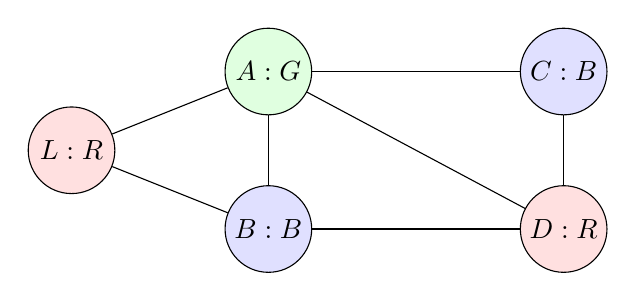
\begin{tikzpicture}[x=1.25cm,y=1cm,
every node/.style={draw,circle,minimum size=11mm,inner sep=2pt}]
\node[fill=red!12] (L) at (0,0) {$L:R$};
\node[fill=green!12] (A) at (2,1) {$A:G$};
\node[fill=blue!12] (B) at (2,-1) {$B:B$};
\node[fill=blue!12] (C) at (5,1) {$C:B$};
\node[fill=red!12] (D) at (5,-1) {$D:R$};
\foreach \u/\v in {L/A,L/B,A/B,A/C,A/D,B/D,C/D}
\draw (\u)--(\v);
\end{tikzpicture}
\end{center}
All seven edges join different colors.

\section*{CSP3 (p.\ 3)}
Write SA = South Australia, Q = Queensland,
NSW = New South Wales, V = Victoria,
WA = Western Australia, NT = Northern Territory.

In the modified map, Victoria extends along the east side of NSW
and shares a border with Queensland. Thus SA, Q, NSW, V are
pairwise adjacent:
\[
\{SA\!-\!Q,\ SA\!-\!NSW,\ SA\!-\!V,\ Q\!-\!NSW,\ Q\!-\!V,\ NSW\!-\!V\}.
\]
\begin{center}
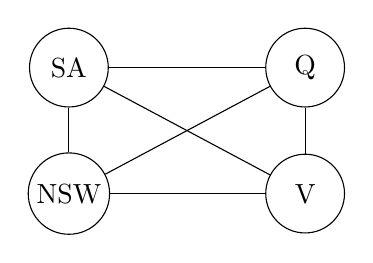
\begin{tikzpicture}[x=1cm,y=.8cm,
every node/.style={draw,circle,minimum size=10mm,inner sep=2pt}]
\node (SA) at (0,1) {SA}; \node (Q) at (3,1) {Q};
\node (NSW) at (0,-1) {NSW}; \node (V) at (3,-1) {V};
\foreach \u/\v in {SA/Q,SA/NSW,SA/V,Q/NSW,Q/V,NSW/V}
\draw (\u)--(\v);
\end{tikzpicture}
\end{center}
These four regions form $K_4$. With only three colors, at least two
would have the same color, contradicting their adjacency. Therefore
$\chi\ge4$.

Four colors also suffice. One valid coloring is
\[
\begin{array}{c|cccccc}
\text{Region}&WA&NT&SA&Q&NSW&V\\ \hline
\text{Color}&2&3&1&2&3&4
\end{array}
\]
Every neighboring pair has different colors. Hence $\chi\le4$, and
\[
\boxed{\chi=4}.
\]
\end{document}
